\begin{enumerate}
\item 	\begin{ljrp}\runningj \nonet โดยปกติเข็มทิศจะวางตัวตามแนวทิศเหนือ - ใต้  เมื่อนำเข็มมาวางใกล้ ๆ กับกึ่งกลางแท่งแม่เหล็กที่ตำแหน่งดังรูป  เข็มทิศจะชี้ในลักษณะใด
    \begin{2c}
        {\begin{adjustbox}{valign=t}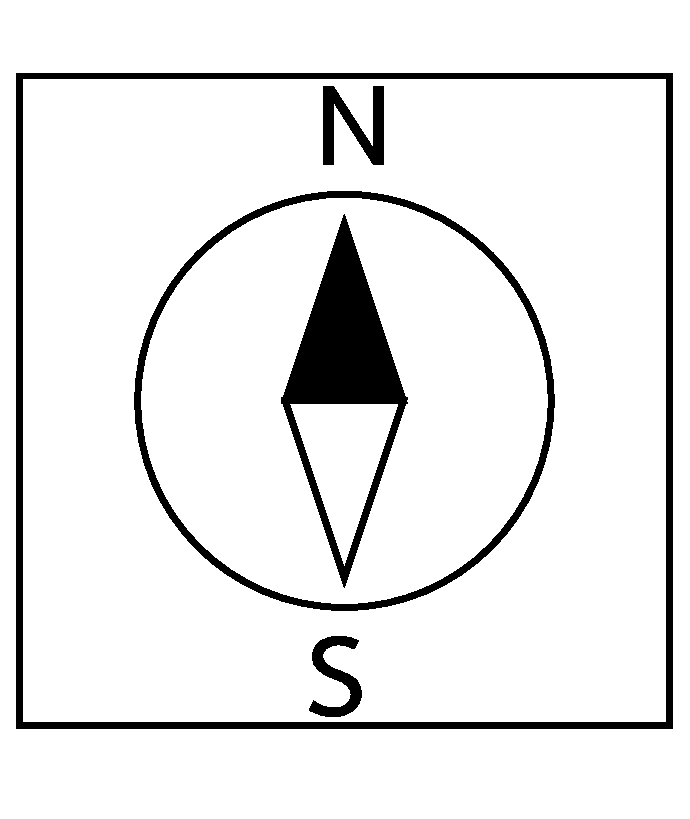
\includegraphics[width=2cm]{l2j-2-2.eps}\end{adjustbox}}
        {\begin{adjustbox}{valign=t}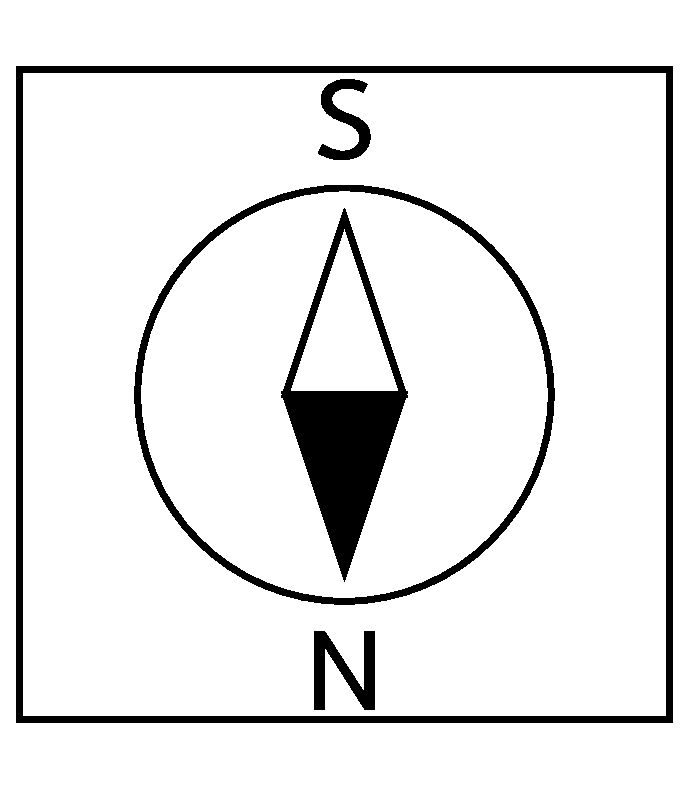
\includegraphics[width=2cm]{l2j-2-3.eps}\end{adjustbox}}
        {\begin{adjustbox}{valign=t}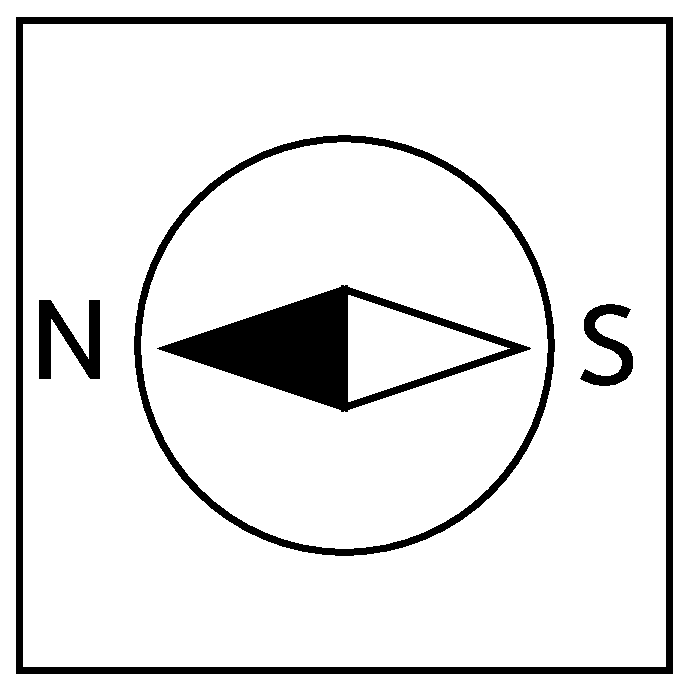
\includegraphics[width=2cm]{l2j-2-4.eps}\end{adjustbox}}
        {\begin{adjustbox}{valign=t}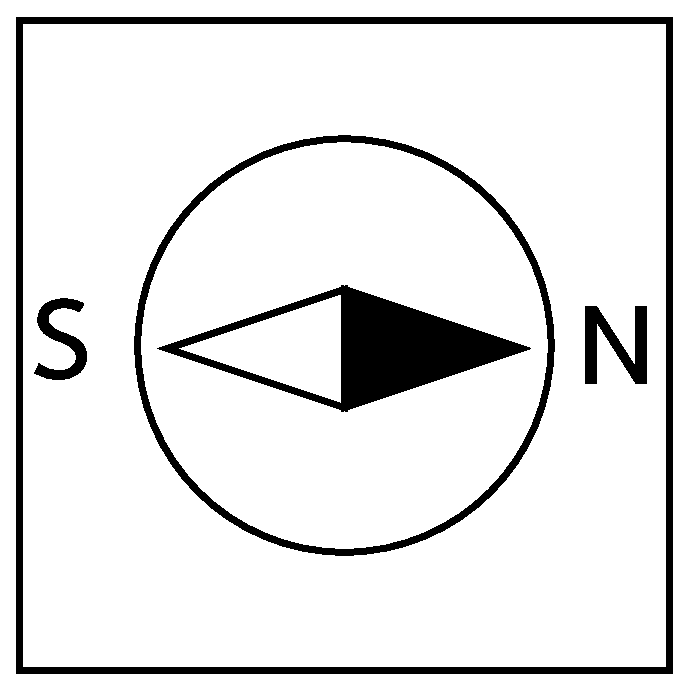
\includegraphics[width=2cm]{l2j-2-5.eps}\end{adjustbox}}
    \end{2c} 
		\end{ljrp}
		\begin{rp}{l2j-2-1.eps}\end{rp}
\end{enumerate}



